\clearpage
\chapter{Conclusion}

\section{Final Remarks}

In this paper, a serial implementation of the FEM was completed to solve a generic PDE problem posed used C++11. The code was partitioned into three main sections, the mesh generation, assembling the global stiffness matrix, and solving the  linear system. The mesh generation and application of the FEM were written using classes and some of C++11 STL features. The linear solver for the global system was implemented using Intel's MKL solver libraries. This serial version of the FEM was written to work for both sparse and dense global stiffness matrices and the assembly portion came in two different variants, applying DSS and LAPACKE for the solving portion, respectively. A sparsity scanner had to be implemented as part of the Mesh class in order to a priori deduce the sparsity pattern of the resulting FEM, so as to be able to assemble the CSR matrix. This was done using graph theory logic and using STL's sets. Both implementations were profiled to deduce the most dominant kernel in the process and tested up to problem sizes of 40,000 unknowns for the dense case and 490,000 for the sparse. In all cases, the solver resulted in being by a long stretch the most computationally expensive kernel. The results of the code were compared against analytical solutions found in Wolfram Mathematica. The code was timed to see how much of an improvement was seen by applying a sparse solution over a dense and it was seen that Intel's DSS was extremely efficient, taking around 2000~ms to solve for 40,000 unknowns, compared to 500,000~ms for the dense. The sparse solver also saw far more impressive linear scaling compared to the dense solver's quadratic - indicating that the speed-ups would only grow as problem size got larger.

The FEM implementations were then investigated for potential scope for parallelisation an naive sparse and dense implementations were then ported onto CUDA code for running on Nvidia's GPUs. There were many considerations taken when performing the port, such as thread divergence, optimising shared memory usage and reducing over-synchronisation. The main CUDA code purpose-written was for optimising and parallelising the generation of the element matrices and assembly of the global stiffness matrices. The solvers, again, were taken from pre-existing libraries. For the naive CUDA implementation, three solver variants were used, taken from Nvidia's cuSPARSE and cuSOLVER - one which solves a CSR, one which converts from dense to CSR and solves, and finally a dense solver. These were tested and timed for various different problem sizes and block sizes against their corresponding serial versions. Overall, again for the CUDA version, the solvers were the most dominant kernel - in this case even more so, achieving up to 99.5\% computation time. Nvidia's CSR solver did not perform as well as Intel's DSS, showing actual slowdown, while the dense solver outperformed its serial version with speed-ups of around $50\times$. 

It was noted after the first prototype of the code that there was a large portion of thread register usage and so an optimisation strategy was implemented to reconfigure the proportion of on-chip memory allocated to registers or shared memory. This saw no difference to the solver times, but did see improvements in the generation of the element matrices and assembly of the global system steps. These both saw huge speed-ups over the serial code, with the element matrices seeing $5000\times$ and the assembly seeing $20000\times$ and $120000\times$ times for the sparse and dense cases, respectively. Other profiling was done such as timing allocation and transfer time to check if the scaling is as should be expected given the memory needed - which it was shown to be. Profiling was also done on NVVP to show a minimal effect of warps causing thread divergence, and the improvement in memory usage, as well as the main contributing stall factors and the load distribution.

The next step taken in this report was the write the novel FEM Single Element Solution (FEMSES) implementation - which removes the assembly step from the traditional FEM and applies a Jacobi relaxation scheme on the local element solutions instead. Again, careful considerations like above had taken when implementing the code in CUDA due to GPU limitations. The code was structured into four main constituent kernels, one to generate the element matrices and store them in global memory, one to apply the Jacobi iteration, one to assemble the global solution estimate and finally one to evaluate the 2-norm of the error in the current iteration. The last kernel made use of pre-existing cuBLAS functions to calculate the error. Again, the code was timed and profiled to deduce performance factors. Overall the FEMSES approach didn't see the same speeds demonstrated in Fernandez~\cite{femses}. It did outperform and scale better than the dense serial case and also had an positive trend for against the naive GPU dense case. In both sparse cases, however, it was outperformed. This was down to poor convergence more so than poorly performing code, as seen in the reasonably good timings when the problem size is small and the convergence rate low. It is suspected this was due to the choice of PDE causing propagation from only two boundaries but this has yet to be tested. This FEMSES implementation was also profiled using NVVP showing good load balance, no thread divergence and a mixed collection of reasons for latencies.

The final thing tested, within the time constraints of this report, was comparing the speeds of the two different cards in the test-bed architecture. All of the previous timings were completed on a Tesla~K40 as the newer RTX~2080 Super had yet to be installed. Once this was, however, the two were compared for timings. The Tesla was outperformed in most of the tests barring the FEMSES implementation. This is potentially down to the fact that the newer cards might have optimised Nvidia's existing libraries better, whereas the FEMSES approach was written on a Tesla and solely tested prior to that on the Tesla and so wasn't written to be optimised on the RTX~2080 Super. That being said, there was some quite positive speed-ups, in some cases reaching double digits.

Concluding then, in investigations in this paper saw a mixed collection of results. In the instances of dense cases, the overall results were quite positive and all showed very positive scaling. For the sparse cases, however, the dominance of the solver portion of the FEM overshadowed the speed-ups seen in the other steps due to the blistering performance of Intel's DSS dominating Nvidia's solver and the FEMSES solver. 

\section{Future Work}

\begin{figure}
	\centering
	\begin{subfigure}{0.35\linewidth}
		\centering
		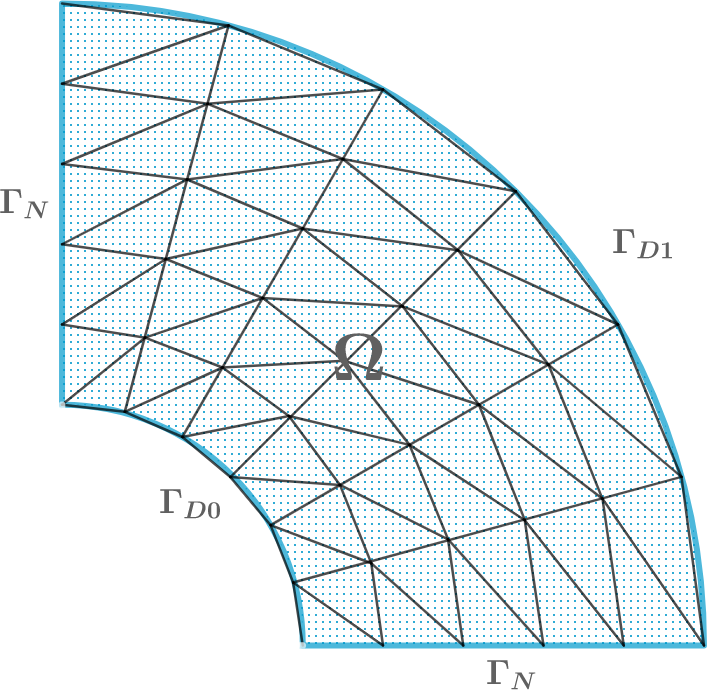
\includegraphics[width = \linewidth]{Figures/annulus}
		\caption{Annulus domain of initially proposed PDE.}
		\label{fig:annul_dom}
	\end{subfigure}\hfill
	\begin{subfigure}{0.53\linewidth}
		\centering
		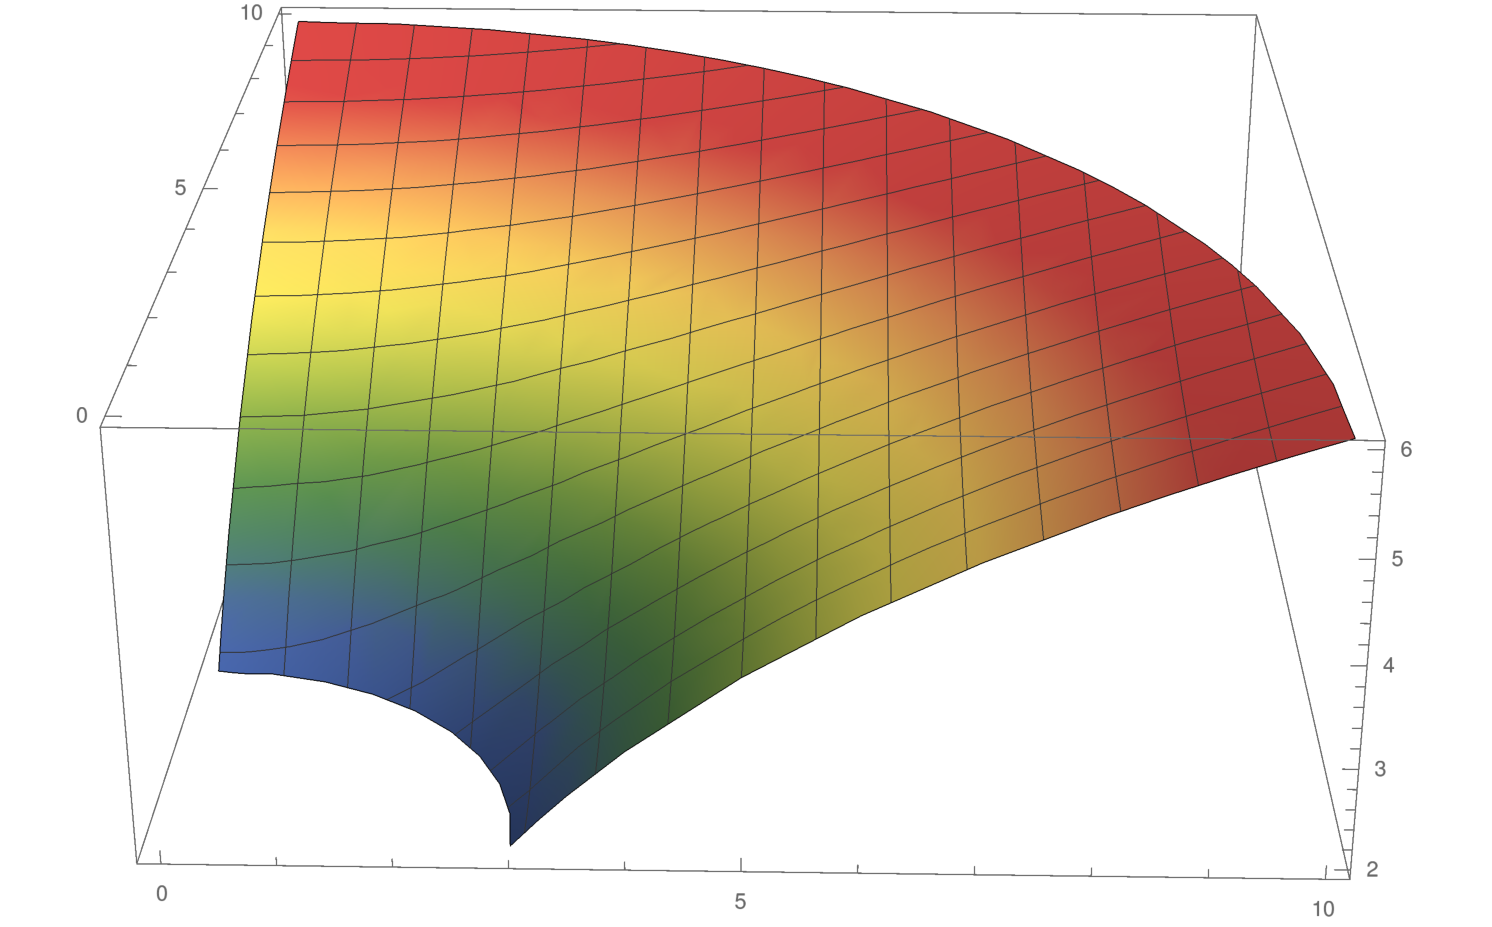
\includegraphics[width=\linewidth]{Figures/annul}
		\caption{Solution from Mathematica of initially proposed PDE..}
		\label{fig:annul_sols}
	\end{subfigure}
	\caption{Domain and solution of initially proposed PDE.}
	\label{fig:init_pde}
\end{figure}

There are still many things to consider at the end of this report - almost endless in reality when it comes to GPU programming. However, there are a few points that would be rather interesting to further investigate if time was permitting. The first one of note is, when coding the serial implementation, the initial plan was to use a PDE with a relatively unusual mesh, such as the one seen in Figure~\ref{fig:init_pde} - since robustness in mesh shape is one of the biggest benefits of choosing the FEM over the finite difference. There wasn't an aim to pick an overly complicated PDE since the purpose of the paper was to test performances, but an interesting mesh like an annulus would have done nicely. It was noted, however, that when using the formulae in Section~\ref{problem}, that in Davies~\cite{davies}, there appeared to have been some assumption made that wasn't clear, that these only work when the cells are all of equal size. It would be a good expansion on the paper to add some numerical integration to evaluate the element matrices instead of those formulae - which would solve the issue of the varying cell size causing problems. The code for the annulus transformation is still in the implementation for future tests. It would even be a nice possibility to add dynamic parallelism to perform the numerical integration on the CUDA implementations.

Another point of potential further study, and probably the most important to this paper, in reality, is to deduce the reason behind the poor rate of convergence for FEMSES compared to in its original literature. The thinking at the time of writing is, since the PDE chosen was a Laplace, which has a sparse RHS vector barring boundary condition enforcements, the propagation from the boundary conditions could be a large factor in the rate of convergence. In this paper, only two of the boundaries were non-homogeneous, resulting in propagation from only two directions. Without yet, of course, having the chance to test this, if a PDE were chosen which has a domain causing it to propagate from more directions, like the one in the FEMSES paper, this might show improved rates of convergence.

If this investigation into the convergence proved fruitful, a next step would be to implement the other FEM GPU implementation discussed, the domain decomposition and multigrid techniques. It would be interesting to see how a fully functioning FEMSES would compare to a method as efficient as multigrid. On top of this, furthering on from not only improving the naive implementation, but with a working FEMSES, an interesting further development would also be to use a different iterative relaxation to Jacobi - which traditionally has poor convergence anyway. This could prove tricky however, given that the input vector and output vector for this semi-Jacobi method are not actually the same, but one rather is a global solution portion and one the local solution. Some consideration would need to go into how to port this even to something like Gauss-Seidel where the most recent update is needed - which would involve the assembly of the global solution estimate at each row in the given iteration.

One final last point for further study that would be important to address is the dominance of the linear solvers - in both computation time and also memory allocation. The choice to use pre-existing solver libraries was done both for convenience and for expected efficiency given the amount of optimisations put into them. However, most of the libraries used direct solvers. These are not optimal for sparse matrices and also, when running took orders more memory. For a case where the amount of memory allocated to the GPU was 208~Mb for the mesh and matrices, Nvidia's cuSOLVER allocated 10.8~Gb to perform its linear solver - this would not happen for iterative methods. It would be good to see how something like the preconditioned Conjugate Gradient method would perform against its serial counterpart.